\begin{frame}
\frametitle{An unsupervised method}

\begin{itemize}
\item An obvious way to segment the sequence is using a threshold value. 
      However, the choice of threshold is difficult in an unsupervised 
      system.
\end{itemize}

\pause
A simple unsupervised method: segment at peaks/valleys.

\vspace{5mm}
\begin{center}
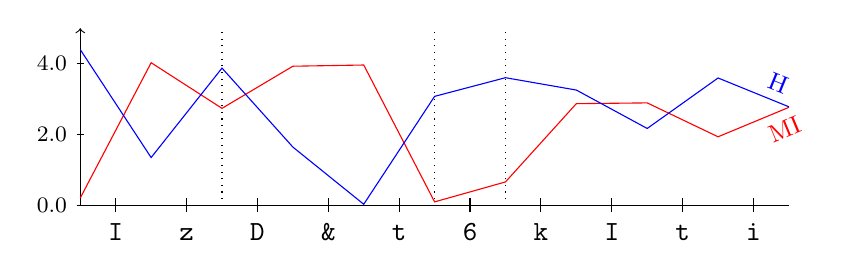
\begin{tikzpicture}[scale=0.45]
\draw (1, -1)  node[anchor=base] {\texttt{I}};
\draw (3, -1)  node[anchor=base] {\texttt{z}};
\draw (5, -1)  node[anchor=base] {\texttt{D}};
\draw (7, -1)  node[anchor=base] {\texttt{\&}};
\draw (9, -1)  node[anchor=base] {\texttt{t}};
\draw (11, -1) node[anchor=base] {\texttt{6}};
\draw (13, -1) node[anchor=base] {\texttt{k}};
\draw (15, -1) node[anchor=base] {\texttt{I}};
\draw (17, -1) node[anchor=base] {\texttt{t}};
\draw (19, -1) node[anchor=base] {\texttt{i}};

\draw (0.0, 0.0) -- (20, 0.0);
\foreach \x in {1,3,...,19} 
   \draw (\x,-0.2) -- (\x,0.2);

\draw[->] (0.0, 0.0) -- (0.0, 5.0);
\draw (-0.1, 4.0) node[left]  {\footnotesize 4.0} -- (0.1, 4.0);
\draw (-0.1, 2.0) node[left] {\footnotesize 2.0} -- (0.1, 2.0);
\draw (-0.1, 0.0) node[left]  {\footnotesize 0.0} -- (0.1, 0.0);
%\draw[red]
%(0, 0.19)    -- (2, 2.80)    -- (4, 2.20)    -- (6, 3.26)    --
%(8, 2.59)    -- (10, 0.16)   -- (12, 0.81)   -- (14, 0.90)   --
%(16, 1.94)   -- (18, -0.15)  -- node[above right,sloped] {\small MI} (20, 1.71)  ;

\draw[red]
(0, 0.209307) --
(2, 4.026254) --
(4, 2.739010) --
(6, 3.927835) --
(8, 3.961770) --
(10,0.098864) --
(12,0.662022) --
(14,2.870927) --
(16,2.892834) --
(18,1.936144) -- node[below right,sloped] {\small MI}
(20,2.767161);

\downtriangle{(4, 2.739010)}{red};
\downtriangle{(10,0.098864)}{red};
\downtriangle{(18,1.936144)}{red};

%\downtriangle{(4, 2.20)}{red};
%\downtriangle{(10, 0.16)}{red};
%\downtriangle{(18, -0.15)}{red};

\draw[blue]
(0, 4.396744) --
(2, 1.350297) --
(4, 3.874525) --
(6, 1.646327) --
(8, 0.032208) --
(10,3.076847) --
(12,3.603842) --
(14,3.255089) --
(16,2.170968) --
(18,3.595810) --  node[above right,sloped] {\small H}
(20,2.782207);

\uptriangle{(4, 3.874525)}{blue};
\uptriangle{(12,3.603842)}{blue};
\uptriangle{(18,3.595810)}{blue};


%\filldraw[blue] (3.85, 3.96) -- (4.0, 4.26) -- (4.15, 3.96) -- cycle;
%\filldraw[blue] (9.85, 4.21) -- (10, 4.51) -- (10.15, 4.21) -- cycle;
%\filldraw[blue] (13.85, 3.97) -- (14, 4.27) --  (14.15, 3.97) -- cycle;
%\filldraw[blue] (17.85, 4.21) -- (18, 4.51) --  (18.15, 4.21) -- cycle;


%\draw[blue,dashed]
%(0, 4.39)   -- (2, 3.16)   -- (4, 4.06)   -- (6, 2.50)   --
%(8, 2.90)   -- (10, 4.31)  -- (12, 3.96)  -- (14, 4.07)  --
%(16, 3.16)  -- (18, 4.31)  -- node[above right,sloped] {\small H} (20, 4.03) ;

     
\foreach \x in {4,10,12} 
   \draw[dotted] (\x,-0.4pt) -- (\x,5);
\end{tikzpicture}
% MI <2,1>
%<<I,0.209307 
%<Iz,4.026254 
%IzD,2.739010 
%zD&,3.927835 
%D&t,3.961770 
%&t6,0.098864 
%t6k,0.662022 
%6kI,2.870927 
%kIt,2.892834 
%Iti,1.936144 
%ti>,2.767161 

% H <2,1>
%<<I,4.396744
%<Iz,1.350297
%IzD,3.874525
%zD&,1.646327
%D&t,0.032208
%&t6,3.076847
%t6k,3.603842
%6kI,3.255089
%kIt,2.170968
%Iti,3.595810
%ti>,2.782207
\end{center}

\end{frame}

